\documentclass[a4paper]{article}

\usepackage[utf8]{inputenc}
\usepackage[T1]{fontenc}
\usepackage[spanish]{babel}
\usepackage[margin={20mm,25mm}]{geometry}

\usepackage{ifthen}
\usepackage{mathtools}
\usepackage{xcolor}
\usepackage{booktabs}
\usepackage{circuitikz}
\usepackage{fancyhdr}
\usepackage{parskip}
\usepackage{hyperref}
\usepackage{graphicx}

% --------------------
% DATOS DEL INFORME
\newcommand{\numeroTarea}   {1}                 % <-- Reemplazar X con el número de la tarea
\newcommand{\numeroGrupo}   {22}                 % <-- Reemplazar N con el número de su grupo
\newcommand{\nombrePrimero} {Martín Arancibia Alvarado}    % <-- Reemplazar con el nombre del primer integrante
\newcommand{\rolPrimero}    {201973517-9}        % <-- Reemplazar con el rol del primer integrante
\newcommand{\nombreSegundo} {Miguel Soto Delgado}    % <-- Reemplazar con el nombre del segundo integrante
\newcommand{\rolSegundo}    {201973623-K}        % <-- Reemplazar con el rol del segundo integrante
% --------------------

% --------------------
% NO MODIFICAR ESTA PARTE
\title{Informe Tarea \numeroTarea \\ \large
    \ifthenelse{\equal{\numeroTarea}{1}}{Circuito Combinacional}{}
    \ifthenelse{\equal{\numeroTarea}{2}}{Circuito Secuencial}{}
    \ifthenelse{\equal{\numeroTarea}{3}}{Lenguajes de Descripción de Hardware}{}
    \ifthenelse{\equal{\numeroTarea}{4}}{ARM Assembly}{}
    \ifthenelse{\equal{\numeroTarea}{X}}{Tema de la tarea}{}
}
\author{\textbf{Grupo \numeroGrupo} \\ \begin{tabular}{r @{\quad} l}
    \nombrePrimero & \rolPrimero \\
    \nombreSegundo & \rolSegundo
\end{tabular}}
\date{\today}

\setlength{\parindent}{15pt}
\addto\captionsspanish{\renewcommand{\tablename}{Tabla}}
% --------------------

\begin{document}

\begin{titlepage}
    
    \vfill
    
    \begin{figure}
        
\includegraphics[width=0.3\textwidth]{logo_usm.png} % Con esto pueden incluir imágenes que hayan subido a Overleaf
    \end{figure}

    \maketitle
    % \thispagestyle{empty}
    
    \newpage

    \vfill
    \tableofcontents
\end{titlepage}

\newpage

\section{Desarrollo de la tarea}

\section{Movimiento Básico}

Primero modelamos el movimiento del robot a partir de lo indicado en el enunciado, en donde tomamos las siguientes variables; si el robot tiene más de 3 cargas (B), si hay enemigos a su izquierda, frente o derecha (Ei, Ef, Ed) y finalmente si hay estaciones de carga a su izquierda, frente y derecha (Ci, Cf, Cd) en exactamente ese orden. Todo esto produciendo las distintas salidas; ir a la izquierda, ir al frente e ir a la derecha (L, F, R). Debido a que no existía otras especificaciones a lo largo de la tarea, se asumirán los siguientes supuestos: 

\begin{itemize}

\item En caso de que no hayan unidades de carga ni enemigos, el ExaBot se moverá según la prioridad dada por su estado de carga, es decir, la prioridad que tengan los movimientos vendrán dados por B (Ej: no existe nada en ninguno de los 3 caminos y el robot tiene 2 cargas, por lo que este se moverá hacía adelante).

\item El Exabot siempre intentará moverse, en el caso que haya un camino disponible, esto incluye los casos donde este tiene una carga menor a 3.

\item Como 0 es un número menor que 3, el ExaBot podrá moverse con una carga de 0, incluso en el caso que no existan unidades de carga alrededor. Este caso solo hará que se comporte de igual manera que para el 1, 2 y 3.

\end{itemize}

Para empezar, definiremos los eventos de manera que sean entendibles dentro de los parámetros que nos ofrece la herramienta; la batería (B) tendrá un valor de 0 siempre que su carga sea igual o menor a 3, y un valor de 1 en cualquier otro caso. Esto se logró mediante el siguiente circuito que está insertado a la derecha del input de 4 bits (Input el cual corresponde a la carga actual). 

%Aqui viene la imagen del circuito que viene de la bateria.

\begin{center}
    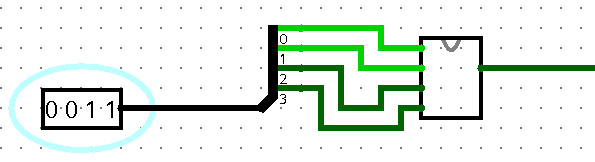
\includegraphics[width=0.7\textwidth]{tarea-1-carga-ej-1.png} % Con esto pueden incluir imágenes que hayan subido a Overleaf
    \\
    En este caso, la batería tiene un nivel de carga igual a 3, por ende su salida es 0.
\end{center}

\begin{center}
    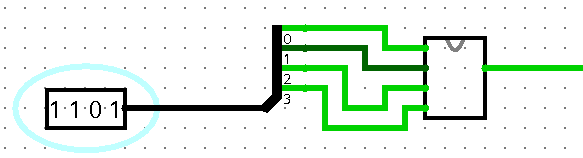
\includegraphics[width=0.7\textwidth]{tarea-1-carga-ej-2.png} % Con esto pueden incluir imágenes que hayan subido a Overleaf
    \\
    En este otro caso, el nivel de la batería es 13, teniendo una salida igual a 1.
\end{center}

Una vez tenemos el estado actual de la batería, tomaremos los 6 pines que se encuentran a la izquierda y haremos inputs válidos (Reconoceremos como input válido cualquier input el cual no ponga en la misma posición una estación de carga y un enemigo) cambiando los valores de estos entre 0 y 1, 0 indicando que no existe un enemigo/estación de carga en esa posición y 1 indicando que existe un enemigo/estación de carga en esa posición. En caso de poner un input inválido la salida será siempre 0 0 0.

%Poner imagen extra del circuito con un input cualquiera.

Ya con todos los datos ingresados al circuito, este revisará, por medio del subcircuito llamado "Circuito Bot", hacía que posición debe moverse nuestro bot dada las condiciones iniciales, y en ese momento saldrá, por medio de alguno de los pines de salida, la dirección tomada por el bot. El pin el cual quede con un 1 nos demarca en que dirección el bot se ha movido.

%Imagen del circuito bot

Haciendo el análisis de este circuito, tendremos que la expresión matemática para el circuito, y se define como:

\begin{center}
    
    \overline{B El Ef} Cl \overline{Cf Cr} + \overline{B El Er} Cl \overline{Cf Cr} + \overline{El} Ef Er \overline{Cl Cf Cr} + B \overline{El Ef Cl} Cf + B \overline{El} Ef \overline{Er Cl Cf}
    \label{eq:ej_ecuacion} % Este es el identificador de la ecuación

\end{center}

Y el circuito completo quedará de la siguiente manera:

%Aqui imagen del circuito completo

\begin{center}
    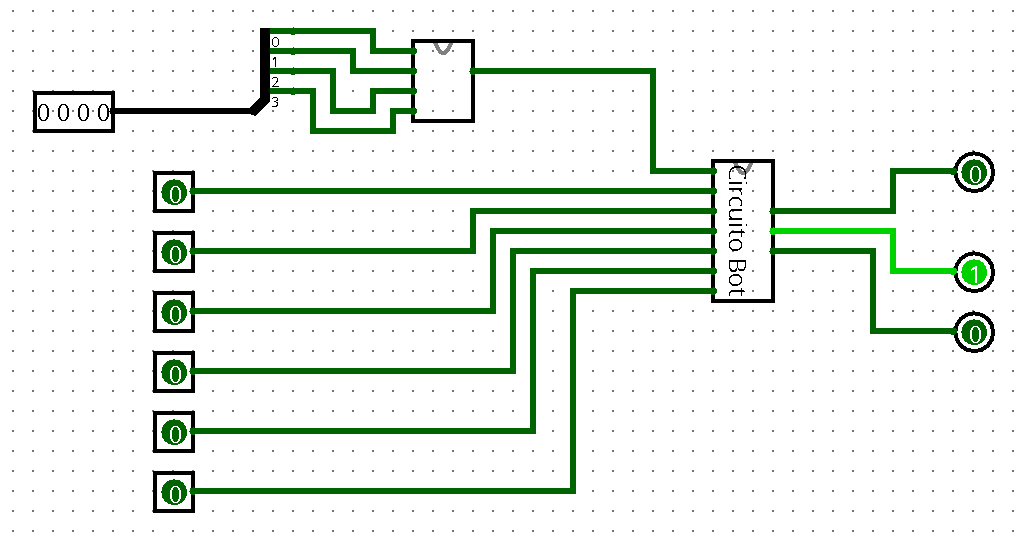
\includegraphics[width=1\textwidth]{tarea-1-main.png} % Con esto pueden incluir imágenes que hayan subido a Overleaf
\end{center}

\section{Estado de Carga}
Para lograr lo anterior, se necesita saber en qué estado de carga está el bot, esto se logró haciendo un circuito para evaluar si se tiene la cantidad de energía necesaria (en este caso más de 3 cargas) o no cumple (tiene 3 o menos cargas). Cómo la batería se mide con una entrada de 4 bits, entonces basta con definir 4 entradas: A, B, C, y D, cada una representando un dígito binario, permitiéndonos modelar los 16 estados posibles de batería del bot. Finalmente, esta dispondrá de una única salida de 1 bit.

La ecuación del estado de la batería se define como:

\begin{equation}
    C + D 
    \label{eq:ej_ecuacion} % Este es el identificador de la ecuación
\end{equation}

Ya que solo nos interesa que el número de carga sea 4 o superior, así que en binario se toma el tercer o cuarto elemento de los cuatro bits.


\begin{center}
    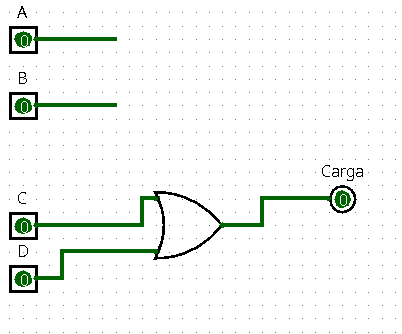
\includegraphics[width=0.6\textwidth]{tarea-1-bat.png} % Con esto pueden incluir imágenes que hayan subido a Overleaf
\end{center}

\section{Resultados y análisis}
Para corroborar que el circuito del robot funciona acorde a la tarea, usamos los ejemplos presentes en el enunciado de la tarea, los cuales son los siguientes:

\begin{center}
    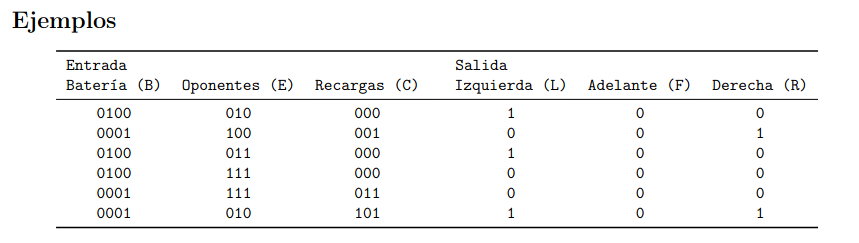
\includegraphics[width=1\textwidth]{tarea-1-ej.png} % Con esto pueden incluir imágenes que hayan subido a Overleaf
\end{center}

En díchos casos, nuestros resultados fueron los siguientes:
\\
\begin{center}
    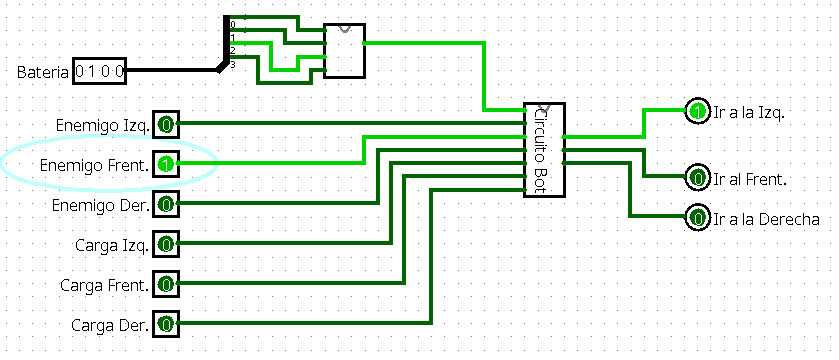
\includegraphics[width=1\textwidth]{tarea-1-ej-1.png} % Con esto pueden incluir imágenes que hayan subido a Overleaf
\end{center}
\begin{center}
    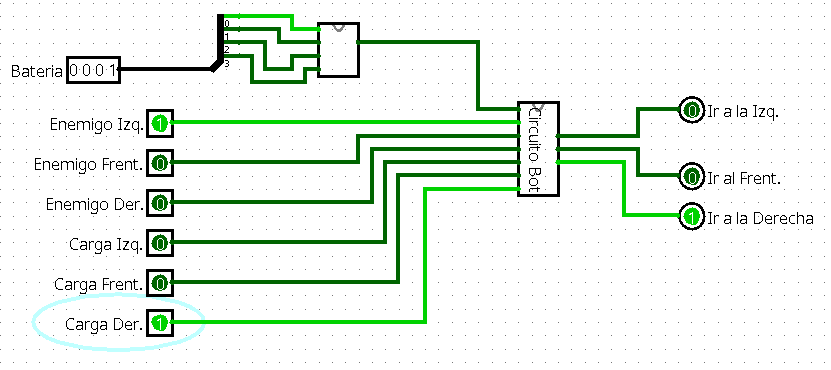
\includegraphics[width=1\textwidth]{tarea-1-ej-2.png} % Con esto pueden incluir imágenes que hayan subido a Overleaf
\end{center}
\begin{center}
    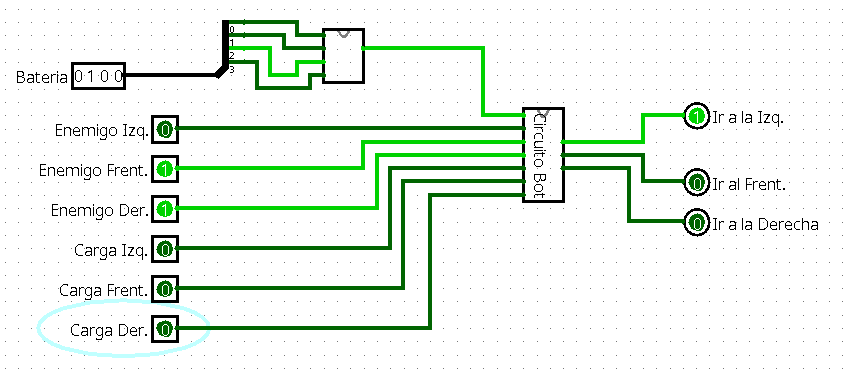
\includegraphics[width=1\textwidth]{tarea-1-ej-3.png} % Con esto pueden incluir imágenes que hayan subido a Overleaf
\end{center}
\begin{center}
    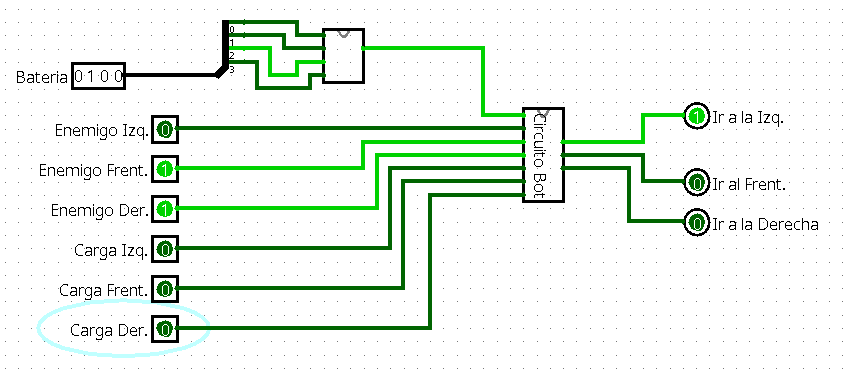
\includegraphics[width=1\textwidth]{tarea-1-ej-3.png} % Con esto pueden incluir imágenes que hayan subido a Overleaf
\end{center}
\begin{center}
    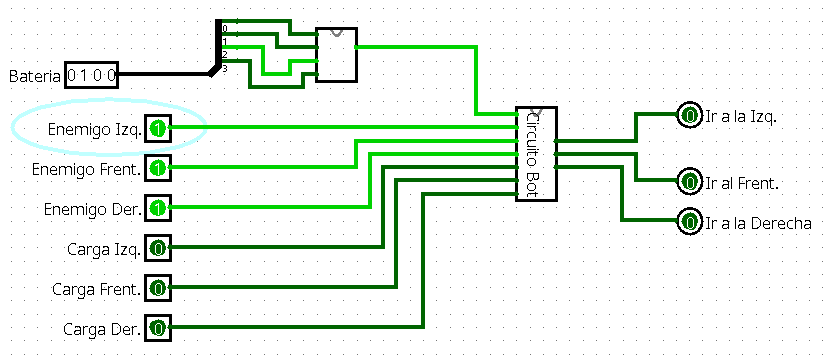
\includegraphics[width=1\textwidth]{tarea-1-ej-4.png} % Con esto pueden incluir imágenes que hayan subido a Overleaf
\end{center}
\begin{center}
    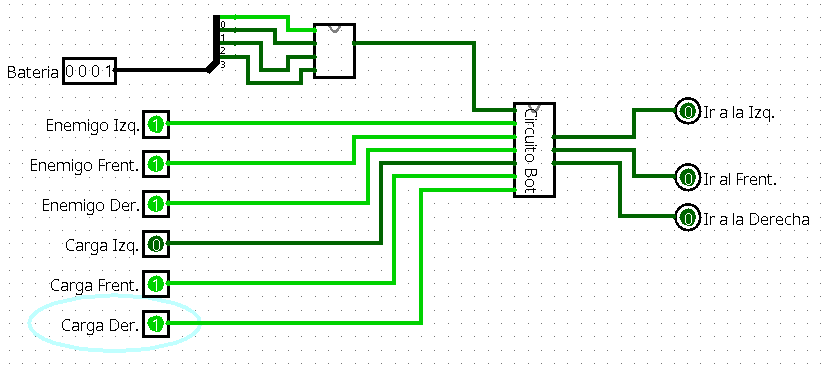
\includegraphics[width=1\textwidth]{tarea-1-ej-5.png} % Con esto pueden incluir imágenes que hayan subido a Overleaf
\end{center}
\begin{center}
    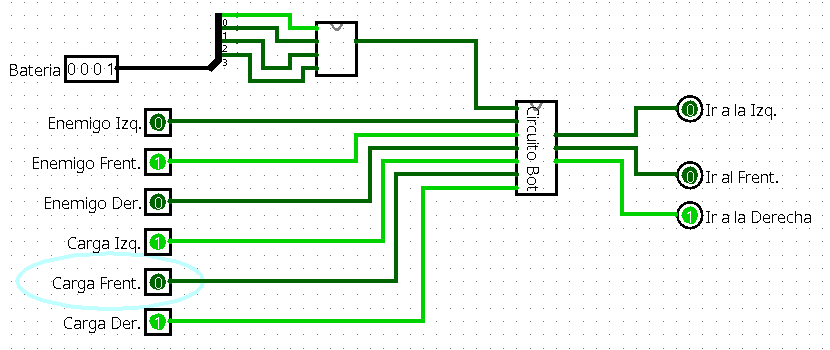
\includegraphics[width=1\textwidth]{tarea-1-ej-6.png} % Con esto pueden incluir imágenes que hayan subido a Overleaf
\end{center}
Al ver los casos en comparación al enunciado, notamos que solo el sexto caso difiere del resultado presentado. Esto se justifica, ya que el enunciado tiene un error, ya que el resultado debiese ser solo una de las direcciones presentadas. En nuestro caso el bot opta por ir a la derecha, porque dicha dirección tiene prioridad por sobre la izquierda al estar con el nivel de carga inferior o igual a 3.
\\\\
También a la hora de realizar el análisis lógico nos percatamos de que el circuito que representa el movimiento del bot era bastante complejo, ya que al poseer 7 entradas diferentes la cantidad de casos posibles subió exponencialmente (siendo la cantidad de casos igual a $2^7 = 128$), dado esto nosotros decidimos no incluir dicha tabla dentro del desarrollo de la tarea y optamos solo por mostrar la operación lógica que describe dicho movimiento.
\\\\
Otro incidente notable es que existían ciertos casos que (al menos bajo nuestra interpretación del problema) eran imposibles, en estricto rigor, aquellos casos en donde había más de un obstáculo en una misma posición. Para estos casos, optamos por asumir que el robot no se movería, debido a que no calza con ninguna de las condiciones mencionadas.
\\\\
Más allá de esto, decidimos incluir otros casos más que sean consistentes con la lógica del movimiento del robot. En los siguientes casos se espera que el bot no sea mueva, ya sea porque son imposibles o porque se rigen por la lógica de prioridad:
\begin{center}
    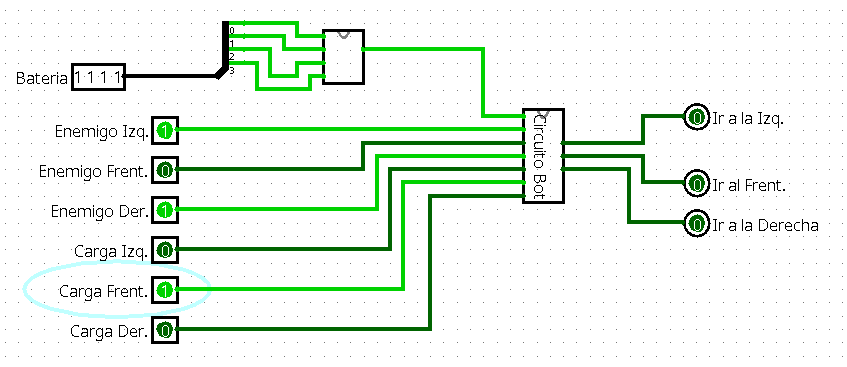
\includegraphics[width=1\textwidth]{tarea-1-ej-7.png} % Con esto pueden incluir imágenes que hayan subido a Overleaf
\end{center}
\begin{center}
    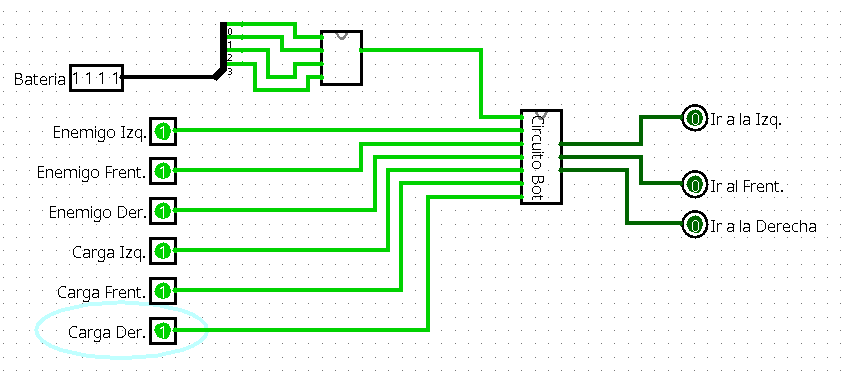
\includegraphics[width=1\textwidth]{tarea-1-ej-8.png} % Con esto pueden incluir imágenes que hayan subido a Overleaf
\end{center}
Finalmente, uno de los casos representados en la figura del enunciado:
\begin{center}
    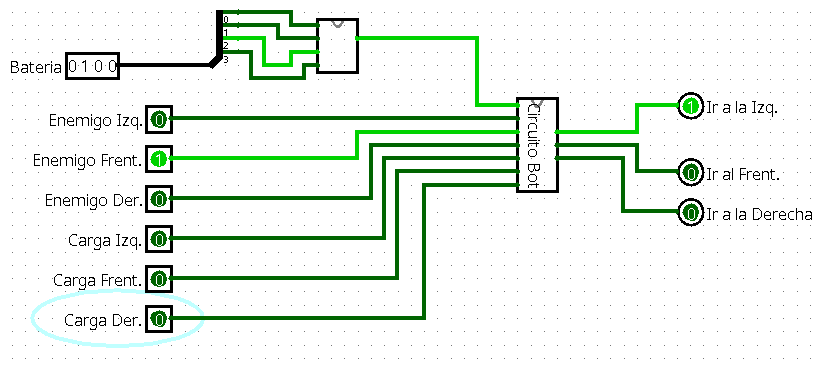
\includegraphics[width=1\textwidth]{tarea-1-ej-9.png} % Con esto pueden incluir imágenes que hayan subido a Overleaf
\end{center}

\section{Conclusiones}
Dando conclusión a este informe, podemos dejar constancia de que se cumplió el objetivo de aprender circuitos combinacionales a través del caso ejemplo proporcionado adjunto a la herramienta "Logisim". A la hora de realizar los análisis pedidos, el software nos facilitó de manera importante la labor, ya que contiene múltiples funcionalidades que hacen más ameno el desarrollo de un circuito que cumpla con las necesidades y parámetros lógicos anticipados.
\\\\
Como grupo, podemos concluir que uno de los mayores problemas que enfrentamos fue el manejo de la tabla porque contenía una cantidad bastante considerable de datos, más allá de eso no tuvimos mayor inconveniente. La experiencia consideramos que fue bastante agradable, esto gracias a que la herramienta nos proporcionó varias facilidades y su naturaleza gráfica hace que una tarea que podría considerarse engorrosa se transforme en un ejercicio entretenido y amigable.

\end{document}
